
\chapter{Stato dell'arte dell'Anomaly Detecion}

\section{Cos'è l'anomaly detection?}


L'Anomaly detection si riferisce al problema di trovare pattern nei dati che non sono conformi al comportamento aspettato. A queste non conformità ci si riferisce come anomalie \cite{anomaly_detection_survey_3}. L'importanza del rilevamento delle anomalie è il fatto che un'anomalia nei dati spesso corrisponde ad un'informazione critica nel dominio a cui si riferisce, per esempio nelle reti di computer un traffico anomalo potrebbe significare che un computer è stato hackerato e sta compiendo azioni per il danneggiamento dell'azienda.

\section{Sfide dell'anomaly detection}

Le anomalie sono definite come un pattern che non rispetta il normale comportamento, ma il definire il concetto di normalità è una sfida, i maggiori fattori che influiscono su questa decisione sono \cite{anomaly_detection_survey_3}:

\begin{itemize}
    \item La difficoltà nel trovare una regione che comprenda tutti i possibili comportamenti normali è molto difficile e il confine tra azioni normali e anomale spesso non è ben definito.
    \item Se le azioni anomale sono generate da azioni malevole, il responsabile cercherà di fare in modo che le osservazioni sui dati appaiano normali.
    \item In alcuni contesti il comportamento si evolve e ciò che è considerato correntemente normale potrebbe essere rappresentativo per il futuro.
    \item È difficile definire quanto la differenza dalla normalità debba essere considerata anomala, per esempio in medicina piccole variazioni per esempio della temperatura corporea possono essere considerate anormali, in finanza la fluttuazione del valore delle azioni potrebbe essere considerato normale.
    \item La disponibilità di dati già classificati come normali o anomali per verificare il modello è uno dei problemi principali.
    \item Spesso i dati contengono rumore che tende ad essere simile alle anomalie ed è difficile rimuoverlo o distinguerlo.
\end{itemize}

\section{Sistemi di rilevamento delle anomalie}



\subsection{Metodo di detection}
% \cite{anomaly_detection_survey_1_network} pagina 24
\begin{itemize}
    \item Classification based
    \item Statistical anomaly detection
    \item Information theory
    \item Clustering-based
\end{itemize}



\subsection{Dati in input}
pagina 6 \cite{anomaly_detection_survey_3}

\subsection{Output of Anomaly Detection}

Un'importante caratteristica è come sono rappresentate le anomalie in uscita dal modello, esistono due metodi: le etichette, tecnica con la quale i dati vengono etichettati con una categoria, tendenzialmente binaria per esempio possiamo etichettare i dati come normali o anomali. L'altro metodo è l'uso di un ``anomaly score'': un punteggio per ogni istanza di dati, che indica quando si discosta dalla normalità, imponendo delle soglie possiamo verificare quali dati sono anomali \cite{anomaly_detection_survey_2_deep_learning,anomaly_detection_survey_3,anomaly_detection_survey_1_network}.

\subsection{Modalità di apprendimento}

I sistemi di classificazione (e gli altri metodi?) necessitano di dataset con esempi di traffico per poter capire in che modo effettuare la classificazione. Per effettuare questo apprendimento esistono tre metodi:

\paragraph{Apprendimento superivisionato}

I sistemi di anomaly detection basati su apprendimento supervisionato hanno prestazioni superiori ai metodi non supervisionati, poichè usano esempi etichettati di dati. I metodi supervisionati imparano il limite di separazione da un set di dati annotato durante una fase di allenamento e successivamente classifica le istanze da testare basandosi sul modello imparato. Avendo bisogno di etichette di difficile reperibilità, questo metodo è poco usato rispetto a quello semi-supervisionato e a quello non supervisionato, ma ha come vantaggi oltre al fatto di essere più preciso anche la velocità della fase di test, basandosi su un modello pre calcolato.
Le tipologie di reti c
% Deep supervised techniques fail to separate normal from anomalous data if the feature space is highly complex and non-linear.

\paragraph{Apprendimento semi-superivisionato}

L'apprendimento semi-supervisionato è una tecnica che che per funzionare assume che tutti i dati usati per l'allenamento siano etichettati in un'unica classe, quella della normalità. Tutte le istanze di dati di dati di test che superano un certo limite intorno alla normalità verranno etichettate come anomale. I vantaggi di questo metodo è che l'uso di dati etichettati può portare ad un grosso miglioramento di performance rispetto alle tecniche non supervisionate, ma rischiano di non essere rappresentative di alcuni casi e sono inclini all'overfitting.
% qua la frase precedente non ha molto senso

\paragraph{Apprendimento non superivisionato}

Questa tecnica si basa su un set di dati normali che contengono che contengono una piccola quantità di dati anomali, l'algoritmo i occuperà di creare un punteggio di separazione basandosi su proprietà intrinseche dei dati.
%magari aggiungere altro pagina 23 \cite{anomaly_detection_survey_2_deep_learning}

\section{Classificazione delle anomalie}

\subsection{Tipologia di anomalie}
Un aspetto importante dell'anomaly detection è l'analisi delle anomalie che possono presentarsi, di conseguenza le anomalie possono essere classificate nel seguente modo:
\begin{itemize}
    \item Anomalie puntuali: un singolo dato che si discosta dalla normalità. Questo è il caso più semplice e su cui si concentra la maggior parte delle ricerche sui dati anomali. Un esempio è un utente che tutti i giorni scarica 1GB di dati quando arriva in ufficio, ma un giorno ne scarica 10.
    \item Anomalie contestuali: quando un insieme di dati si comporta in modo anomalo in un determinato contesto, per esempio il numero di acquisti su un sito durante il periodo di Natale è più alto che durante il resto dell'anno.
    \item Anomalie collettive: quando un'istanza di dati è anormale rispetto all'intero dataset, in questo caso i dati in sè non sono anomali, ma lo diventano quando presi insieme, un esempio è l'elettrocardiogramma, in cui se ci sono bassi valori per un lungo periodo possono identificare un problema.
\end{itemize}

\subsection{Applicazione anomaly detection}
% \subsection{Tipologie anomaly detection}
\begin{itemize}
%todo: dire per ogni tipologia di applicazione quale sistema per l'anomaly detection è usato: esempio nids autoencoders, va, o altro 
%todo: terminare l'elenco delle applicazioni
    \item Fraud detection: sono sistemi con lo scopo di riconoscere frodi, i occupano di rilevare attività illegali in diversi campi come quella assicurativo, finanziario e telefonico.
    \item Medical and Public Health Anomaly Detection: lavorano sui dati dei pazienti, che possono avere anomalie per diverse ragioni: errori di registrazione, errori degli strumenti di misura o una condizione anormale delle condizioni del paziente. Questi sistemi mirano a riconoscere anomalie puntuali usando sistemi semi supervisionati.
    \item Industrial Damage Detection
    \item Image Processing
    \item Anomaly Detection in Text Data
    \item Sensor Networks
    \item Intrusion detection systems(IDS): sono dei sistemi che puntano ad identificare attività malevole nei sistemi informativi, gli IDS possono essere installati su un computer, in quel caso si parla di ``Host Intrusion Detection (HIDS)'' oppure su una rete, in quel caso si parla di ``Network Intrusion Detection (NIDS)'', gli IDS possono essere signature-based oppure anomaly based, nel primo caso non si è in grado di riconoscere nuove tipologie di attacchi. In questo contesto vengono analizzate le anomalie collettive e sono preferiti sistemi di apprendimento semi-supervionato o non supervisionato, perchè le etichette per i dati anomali non sono quasi mai disponibili. In questa tesi mi concentrerò sull'analisi di anomalie di rete basandomi su sistemi di anomaly detection. 
\end{itemize}

\subsection{Tipologia degli attacchi di rete}
%parlare di Network IDS E Host IDS pagina 9 \cite{anomaly_detection_survey_2_deep_learning}
Analizzando 

\section{Le reti neurali}

Spiego cosa sono le reti neurali, come funzionano e come vengono allenate.
\subsection{Funzionamento delle reti neurali}

Le reti neurali sono composte da diversi strati (layer) di nodi, ciascuno collegato al successivo.

L'unità base di ogni rete neurale è il nodo, che rappresenta il neurone artificiale, il tipo base è il ``perceptron'': un nodo con più input e un output rappresentato come una funzione a gradino caratterizzata dalla funzione \ref{eq:perceptron}, in cui si può notare che solo se la sommatoria dei valori in ingresso supera una certa soglia, il neurone si attiva.
%todo: fixare label equazione
\[
\label{eq:perceptron}
output = \begin{cases}
    0 & \mbox{if } \sum_{j}{w_{j}x_{j}}\leq \mbox{threshold} \\
    1 &  \mbox{if } \sum_{j}{w_{j}x_{j}} > \mbox{threshold}
\end{cases}
\]
Questo permette di compiere decisioni in base all'input.
%todo: Per esempio qui posso inserire l'esempio di pagina 3 del libro sulle reti neurali.

\begin{figure}[h]
    % todo: capire come gestire citazioni imsmagini a livello di copyright
    %  e capire come funzionano le label per richiamare le immagini
    \label{fig:neurone}
    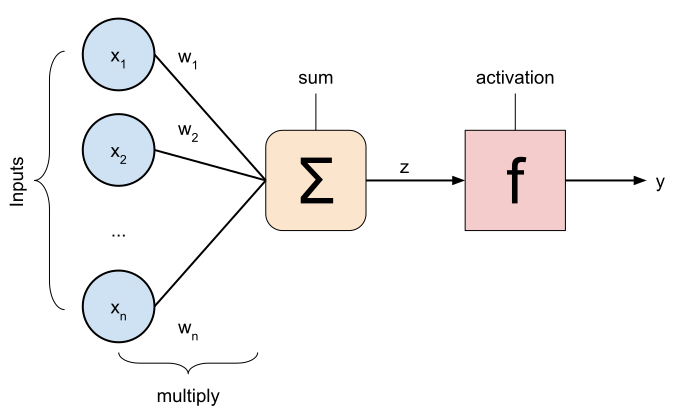
\includegraphics[width=\hsize]{images/reti_neurali/neurone.png}
    \caption{Neurone artificiale}
    \centering
    % https://www.doc.ic.ac.uk/~nuric/teaching/imperial-college-machine-learning-neural-networks.html
\end{figure}

% todo: qua potrei generalizzare dicendo che 
Come si può notare dalla figura con l'evoluzione delle reti neurali non viene più usata solo la funzione a gradino, ma anche delle generiche funzioni rappresentate come ``f''.
Un esempio comunemente usato di evoluzione del perceptron sono i neuroni di Sigmoid, i quali invece di ritornare una funzione a gradino in uscita, ritornano il risultato della funzione di sigmoid ~\ref{eq:sigmoid} \cite{reti_neurali_libro}.

\begin{equation}
    \label{eq:sigmoid}
    \sigma(z) = \frac{1}{1+\mbox{exp}(-\sum_{j}{w_{j}x_{j}} - b)}
\end{equation}
%todo: grafico funzione di sigmoid
Le reti neurali sono composte da gruppi di neuroni artificiali organizzati in livelli e tipicamente composte da almeno tre strati: uno di input, uno o più livelli intermedi definiti ``livelli nascosti'' e un livello di uscita. Ogni livello può contenere uno o più neuroni che possono essere collegati tra loro solo con dei collegamenti in direzione dai nodi di input a quelli di output, in questo caso si parla di ``feedforward'' oppure ``recurrent'' in cui sono previste delle connessioni di feedback a neuroni dello stesso livello o a livelli precedenti.
% 
%https://www.spindox.it/it/blog/ml1-reti-neurali-demistificate/
% fonte immagine https://towardsdatascience.com/what-the-hell-is-perceptron-626217814f53


\subsection{Autoencoders}
\begin{figure}[h]
    % todo: capire come gestire citazioni imsmagini a livello di copyright
    %  e capire come funzionano le label per richiamare le immagini
    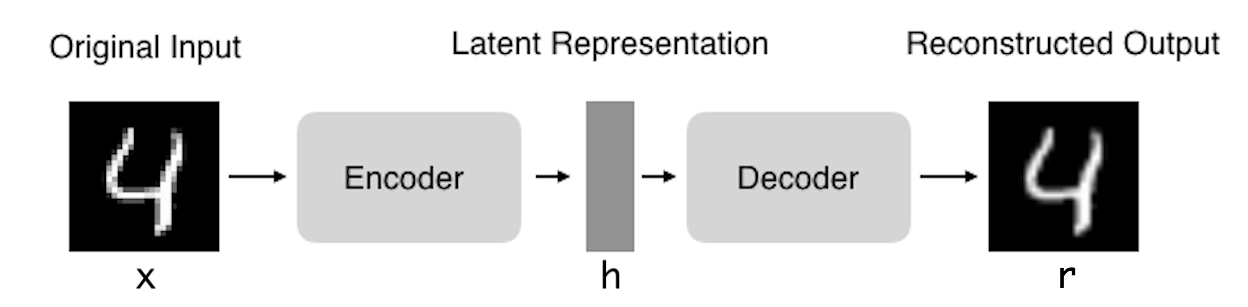
\includegraphics[width=\hsize]{images/reti_neurali/autoencoder.png}
    \caption{Struttura di un autoencoder}
    \label{fig:autoencoder}
    \centering
\end{figure}

%tate of a supercomputer node (lookingat the measured features); afterwards, the model can be used to no-tice representation changes that underlie anomalous conditions. Thishappens because an autoencoder is a neural network trained to copyits input푥to its output푦. Internally it has hidden layersℎencodingthe representation of the data. An autoencoder is composed by twosubparts: an encoding functionℎ=푓(푥)and a decoding function thatreconstructs the input푦=푔(ℎ). Typically, autoencoders do not simplylearn the identity function푔(푓(푥)) =푥but are designed not to beable to copy perfectly, thus the output of an autoencoder is generallydifferent from its input; this difference is calledreconstruction error. Thereconstruction error is used to identify anomalies. During training, anautoencoder learns the relationships among the features in the inputset. If new, previously unseen, data is given to the trained autoencoder
%todo: citare questo articolo https://www-sciencedirect-com.ezproxy.biblio.polito.it/science/article/pii/S0952197619301721

%To reduce overfitting, aDropoutlayer was applied (Srivastava et al.,2014) to the output of layers 1 and 2 (dropout rate equal to 0.2).

Cosa sono gli autoencoder e perchè sono utili nell'anomaly detection.

Gli autoencoder sono una tipologia di reti neurali non supervisionata, anche se quasi sempre vengono usati in maniera semi-supervisionata, che permettono di generare nuovi dati, effettuando in uscita la ricostruzione dei dati forniti in ingresso.
Gli autoencoder sono composti da tre parti, l'encoder, lo spazio latente e il decoder, negli autoencoder la dimensione dell'input è uguale a quella dell'output, e nel mezzo ci sono dei livelli che si occupano prima di comprimere (encoder) le dimensioni, fino a raggiungere lo spazio latente, una forma ``compressa'' dell'input, seguita da una serie di livelli (decoder) che si occupano ti ritornare alle dimensioni originarie ~\ref{fig:autoencoder}.
La capacità di comprimere i dati e decomprimerli si basa sull'allenamento della rete, di conseguenza ogni rete è specifica per una tipologia di dati da comprimere e decomprimere, questo la caratterizza dagli altri sistemi di compressione, per esempio gzip, inoltre è una tipologia di compressione ``lossy'', con perdita, perchè l'uscita sarà simile all'ingresso, ma degradata.
Una popolare applicazione degli autoencoder è l'anomaly detection. Gli autoencoder si occupano di ricostruire i dati iniziali, imparando effettivamente a riprodurre una funzione identità, per questo motivo allenandoli solo con dati di istanze normali quando si troveranno davanti ad un dato anomalo falliranno la ricostruzione dell'input e di conseguenza produrranno un grande errore di ricostruzione \cite{anomaly_detection_survey_2_deep_learning}. 
% https://towardsdatascience.com/applied-deep-learning-part-3-autoencoders-1c083af4d798#f686
% https://www.deeplearningitalia.com/introduzione-agli-autoencoder/

%todo: citare articoli autoencoders
Gli autoencoders sono stati usati da questo, quello e quell'altro ancora per sviluppare questi sistemi di anomaly detection:
\begin{itemize}
    \item articolo 1  \url{https://www-sciencedirect-com.ezproxy.biblio.polito.it/science/article/pii/S0952197619301721}
    \item articolo 2 \url{https://ieeexplore-ieee-org.ezproxy.biblio.polito.it/abstract/document/8363930}
    \item articolo 3 il più importante \url{https://ieeexplore.ieee.org/abstract/document/8438865}
    % \item \url{https://ieeexplore-ieee-org.ezproxy.biblio.polito.it/stamp/stamp.jsp?tp=&arnumber=8336654}
\end{itemize}

\section{Soluzioni esistenti di Anomaly Detection}

Qua illustro delle soluzioni esistenti prese dagli articoli.

\section{Motivazione}
Prova 



